\section{Theoretical Analysis}
\label{sec:analysis}










\begin{equation*}
\begin{bmatrix} 
 0 &      0 & 0 & 1 & 0 & 0 & 0 & 0 \\
1 &      0 & 0 & 0 & 0 & 0 & 0 & 0 \\
G(1) &   -(G(1)+G(2)+G(3)) &     G(2) &    0 &    G(3) &           0 &    0 &    0 \\
0 &      -(G(2)+Kb) &     G(2) &     0 &     Kb &           0 &    0 &    0 \\
-G(1) &    G(1) &   0 &       0 &     G(4)          & 0    & G(6)     & 0 \\
0 &        0 &     0 &    0 &  1 &    0 &    Kd*G(6) & -  1 \\
0 &       -Kb &   
0 &        0 &    0 &        0 &     0 &     0 &    -(G(6)+G(7)) &     G(7) \\
\end{bmatrix}
 \begin{bmatrix} V_1\\V_2\\V_3\\V_4\\V-5\\V_6\\V_7\\V_8 \end{bmatrix} = 
 \begin{bmatrix} 0\\V_s\\0\\0\\0\\0\\0\\0 \end{bmatrix}
\end{equation*}




\begin{table}[H]
  \centering
  \begin{tabular}{|l|r|}
    \hline
    {\bf Name} & {\bf Value [A]} \\ \hline
    \input{../mat/data_alinea_1}
  \end{tabular}
  \caption{Theoretical Values for VOLTAGES using Octave}
  \label{tab:alinea1_voltagens_tab}
\end{table}

%===============================================================
%alinea 2
%===============================================================

\begin{equation*}
\begin{bmatrix} 
   -(G(1)+G(2)+G(3))    & G(2)     & G(3)    &               0    &           0    &             0    &            0\\
          -(G(2)+Kb)    &         G(2)    &   Kb    &                0    &           0    &             0    &            0\\
         G(1)    &     0    &    G(4)    &        0    &          G(6)    &             0    &          0\\
          -Kb    &     0    &    G(5)+Kb    &          -G(5)    &         0    &              0    &          -1\\
           0    &          0    &            1    &          0    &             Kd*G(6)    &     -1               0\\
           0    &     0    &        0    &         1    &            0    &            -1    &            0\\
           0    &       0    &    0    &          0    &      -(G(6)+G(7))    &      G(7)    &     0\\
\end{bmatrix}
 \begin{bmatrix} V_2\\V_3\\V_4\\V-5\\V_6\\V_7\\V_8 \end{bmatrix} = 
 \begin{bmatrix} 0 & 0 & 0 & 0 & 0 & V_6-V_8 & 0\end{bmatrix}
\end{equation*}



\begin{table}[H]
  \centering
  \begin{tabular}{|l|r|}
    \hline
    {\bf Name} & {\bf Value [A]} \\ \hline
    \input{../mat/data_alinea_2}
  \end{tabular}
  \caption{Theoretical Values for VOLTAGES using Octave}
  \label{tab:alinea1_voltagens_tab}
\end{table}

PRESENTAR VALOR DA RESISTENCIA EQUIVALENTE E DA TIME CONSTANT




\begin{figure}[H]
\centering
\includegraphics[width=10 cm]{../mat/natural.eps}
\caption{resposta natural ?=????}
\label{fig:gig_al_2}
\end{figure}





%===============================================================
%alinea 4
%===============================================================


\begin{equation*}
\begin{bmatrix} 
   0 &      0 & 0 & 1 & 0 & 0 & 0 & 0\\
1 &      0 & 0 & 0 & 0 & 0 & 0 & 0\\
G(1) &   -(G(1)+G(2)+G(3)) &     G(2) &    0 &    G(3) &           0 &    0 &    0\\
0 &      -(G(2)+Kb) &            G(2) &     0 &     Kb &           0 &    0 &    0\\
-G(1) &    G(1) &                 0 &       0 &     G(4)          & 0    & G(6)     & 0\\
0 &        0 &                    0 &       0 &      1 &           0 &    Kd*G(6) &  -1\\
0 &        0 &                    0 &        0 &     0 &            0 &    -(G(6)+G(7)) &     G(7)\\
0 &        -Kb &                  0 &         0 &      G(5)+Kb &     -G(5)-y &      0 &         y\\

\end{bmatrix}
 \begin{bmatrix} V_1\\V_2\\V_3\\V_4\\V-5\\V_6\\V_7\\V_8 \end{bmatrix} = 
 \begin{bmatrix} 0 & V_s & 0 & 0 & 0 & 0 & 0 & 0\end{bmatrix}
\end{equation*}


\begin{figure}[H]
\centering
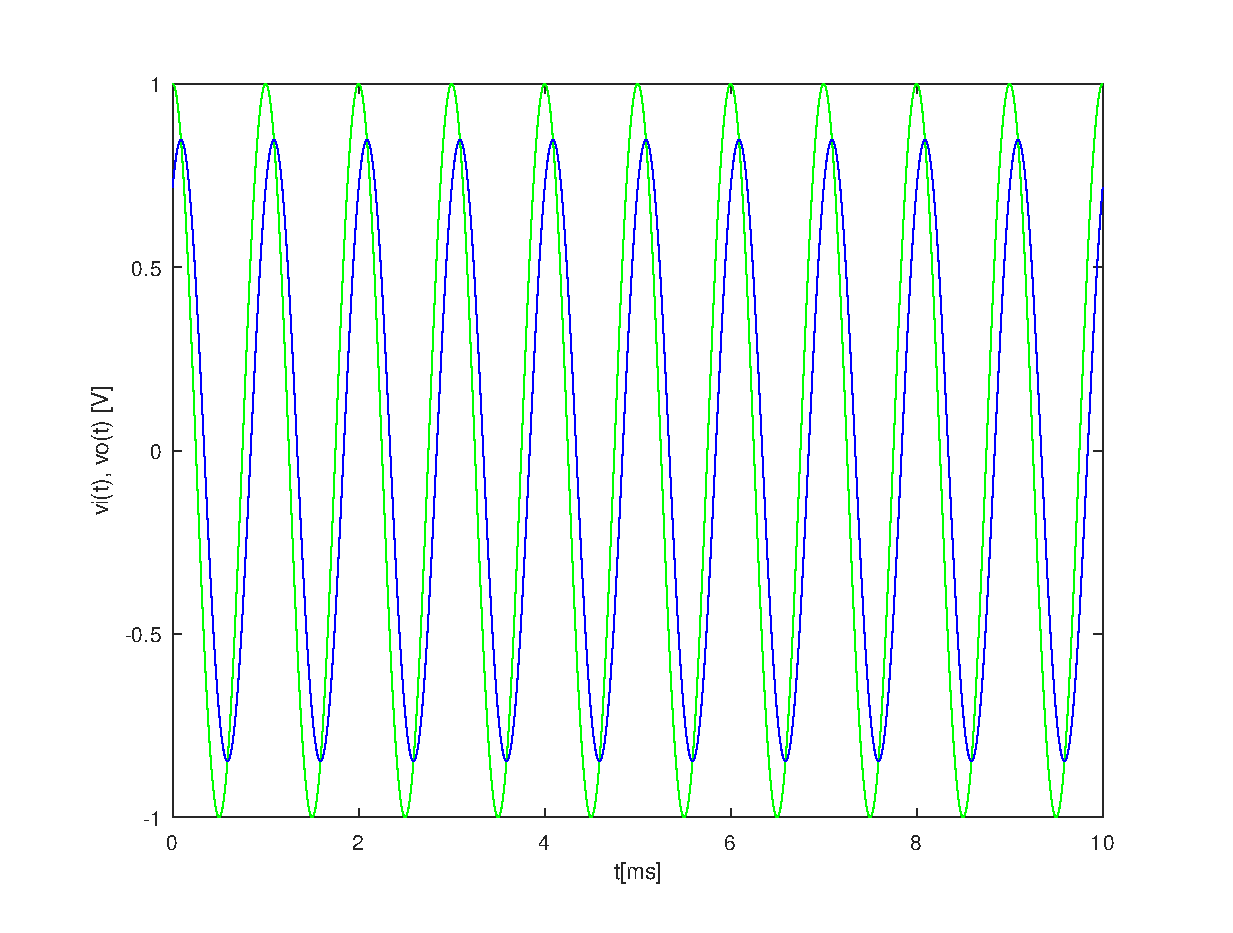
\includegraphics[width=10 cm]{../mat/forced.eps}
\caption{resposta natural ?=????}
\label{fig:gig_al_2}
\end{figure}




\begin{figure}[H]
\centering
\includegraphics[width=10 cm]{../mat/final.eps}
\caption{resposta natural ?=????}
\label{fig:gig_al_2}
\end{figure}
